\chapter{Deep learning}\label{ch-17}

Questa lezione introduce il \textbf{deep learning} (DL) dal punto di
vista del corso: non i dettagli delle architetture per le applicazioni
(che si vedranno nei corsi successivi del curriculum AI, come Pattern
Recognition e NLP), ma una \textbf{visione d'insieme} delle reti con
molti strati, i concetti che le rendono efficaci (\textbf{servono
davvero molti strati?}, \textbf{representation learning},
\textbf{rappresentazioni distribuite}) e le principali \textbf{tecniche}
di addestramento, molte delle quali utili anche nel caso ``base''.

\section{Che cos'è il deep learning}\label{che-cosuxe8-il-deep-learning}

\begin{boxnote}{LeCun, Bengio, Hinton, \emph{Nature} (2015)}

\emph{``Il deep learning permette a modelli computazionali composti da
più strati di elaborazione di apprendere rappresentazioni dei dati con
più livelli di astrazione. Questi metodi hanno migliorato drasticamente
lo stato dell'arte nel riconoscimento del parlato, nel riconoscimento
visivo di oggetti, nel rilevamento di oggetti e in molti altri
domini.''}

\end{boxnote}

\subsection{Un po' di storia}\label{un-po-di-storia}

Dal 2010 circa il deep learning ha avuto un forte impatto
sull'industria, per tre fattori:

\begin{itemize}
\tightlist
\item
  \textbf{grandi dataset} disponibili (milioni di immagini);
\item
  \textbf{potenza di calcolo} (le GPU sono il fattore abilitante);
\item
  \textbf{nuove idee} per facilitare l'addestramento.
\end{itemize}

L'apprendimento con architetture profonde non è più ``infattibile''. I
nuovi risultati allo stato dell'arte nel riconoscimento del parlato,
nella traduzione automatica (Google Neural Translator dal 2016, DeepL) e
nel riconoscimento di immagini hanno attratto moltissimi ricercatori. In
passato ci si aspettava un miglioramento cambiando la scala di modelli e
dati, ma non necessariamente un tale salto di prestazioni. Tutte le
grandi aziende informatiche basano oggi le loro strategie di ricerca e
sviluppo su questi approcci.

\subsection{Il quadro generale}\label{il-quadro-generale}

Il DL è un \textbf{quadro generale} che include modelli diversi:

\begin{itemize}
\tightlist
\item
  \textbf{reti neurali profonde} (MLP con molti strati);
\item
  \textbf{reti convoluzionali} (vincenti in computer vision);
\item
  \emph{deep belief network} e approcci generativi;
\item
  reti \textbf{ricorrenti} e \textbf{ricorsive};
\item
  \ldots{}
\end{itemize}

Si contrappone ai \textbf{modelli ``shallow''} (superficiali), ad
esempio reti con meno di 3 strati. Gli aspetti comuni ai vari approcci
sono:

\begin{itemize}
\tightlist
\item
  \textbf{più strati} di unità di elaborazione \textbf{non lineari};
\item
  apprendimento (supervisionato o non supervisionato) di
  \textbf{rappresentazioni delle feature} in ogni strato, con gli strati
  che formano una \textbf{gerarchia} da feature di basso livello a
  feature di alto livello (diversi livelli di astrazione);
\item
  quindi, una \textbf{rappresentazione gerarchica, sparsa e distribuita}
  dei dati.
\end{itemize}

(Le differenze dipendono dai modelli specifici: max pooling nelle CNN,
addestramento basato sull'energia nelle RBM, ecc.)

\subsection{Gli ingredienti concettuali: astrazione
gerarchica}\label{gli-ingredienti-concettuali-astrazione-gerarchica}

Si ricordi lo XOR risolto con due strati
(\href{06\%20-\%20Reti\%20neurali\%20(parte\%201)\%20-\%20dal\%20neurone\%20al\%20MLP}{06
- Reti neurali (parte 1) - dal neurone al MLP}): lo strato nascosto crea
una \textbf{ri-rappresentazione interna} che rende facile il compito
allo strato di uscita, e questa composizione di operazioni intermedie si
può estendere su molti livelli di astrazione.

\begin{itemize}
\tightlist
\item
  \textbf{Feature learning} non supervisionato o semi-supervisionato ed
  estrazione gerarchica di feature, \textbf{invece del feature
  engineering} (feature estratte a mano, per esperienza, come la texture
  nelle immagini): si passa al concetto di \textbf{apprendere
  rappresentazioni dei dati}.
\item
  \textbf{Livelli di astrazione crescenti} attraverso gli strati.
  Un'immagine si può rappresentare come vettore di intensità dei pixel,
  oppure in modo più astratto come insieme di bordi, regioni di forma
  particolare, ecc.: \textbf{i bordi formano motivi, i motivi si
  assemblano in parti, le parti formano oggetti}\ldots{} su molti
  livelli.
\item
  Funziona al meglio quando l'input ha una qualche forma di
  \textbf{struttura} (spaziale, temporale, \ldots).
\end{itemize}

\begin{figure}[htbp]
\centering
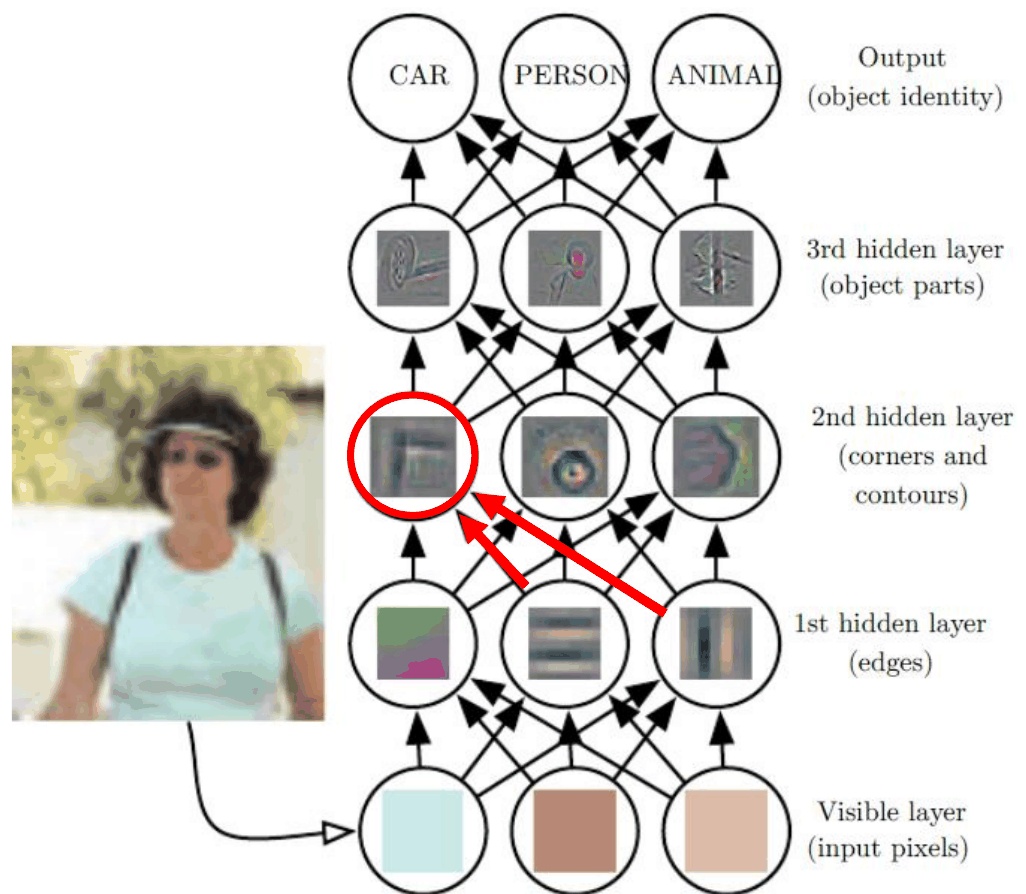
\includegraphics[width=0.63\linewidth,height=0.42\textheight,keepaspectratio]{images/17-deep_gerarchia.png}
\caption{Dai pixel all'identità dell'oggetto: una serie di strati nascosti estrae
feature sempre più astratte (bordi → angoli e contorni → parti di
oggetti).}
\end{figure}

Il deep learning risolve la difficoltà di una mappatura complicata
(pixel → identità) \textbf{scomponendola in una serie di mappature
semplici annidate}, ciascuna descritta da uno strato diverso. La nuova
rappresentazione \textbf{semplifica la classificazione} nell'ultimo
strato. Ci sono analogie con il sistema visivo biologico.

Nelle reti queste feature astratte \textbf{si apprendono dagli esempi}:
con la backpropagation, l'errore sullo strato di uscita (ad esempio per
distinguere auto e persone) si propaga tramite i delta attraverso gli
strati, e le unità si specializzano per fornire feature di alto livello
utili a quello scopo (la ruota per l'auto, la mano per la
persona\ldots). Il legame tra le feature sviluppate automaticamente e la
realtà è un aspetto affascinante; e sorprendentemente i primi filtri
estraggono linee orizzontali o verticali, proprio come farebbe un
semplice filtro convolutivo lineare.

\begin{figure}[htbp]
\centering
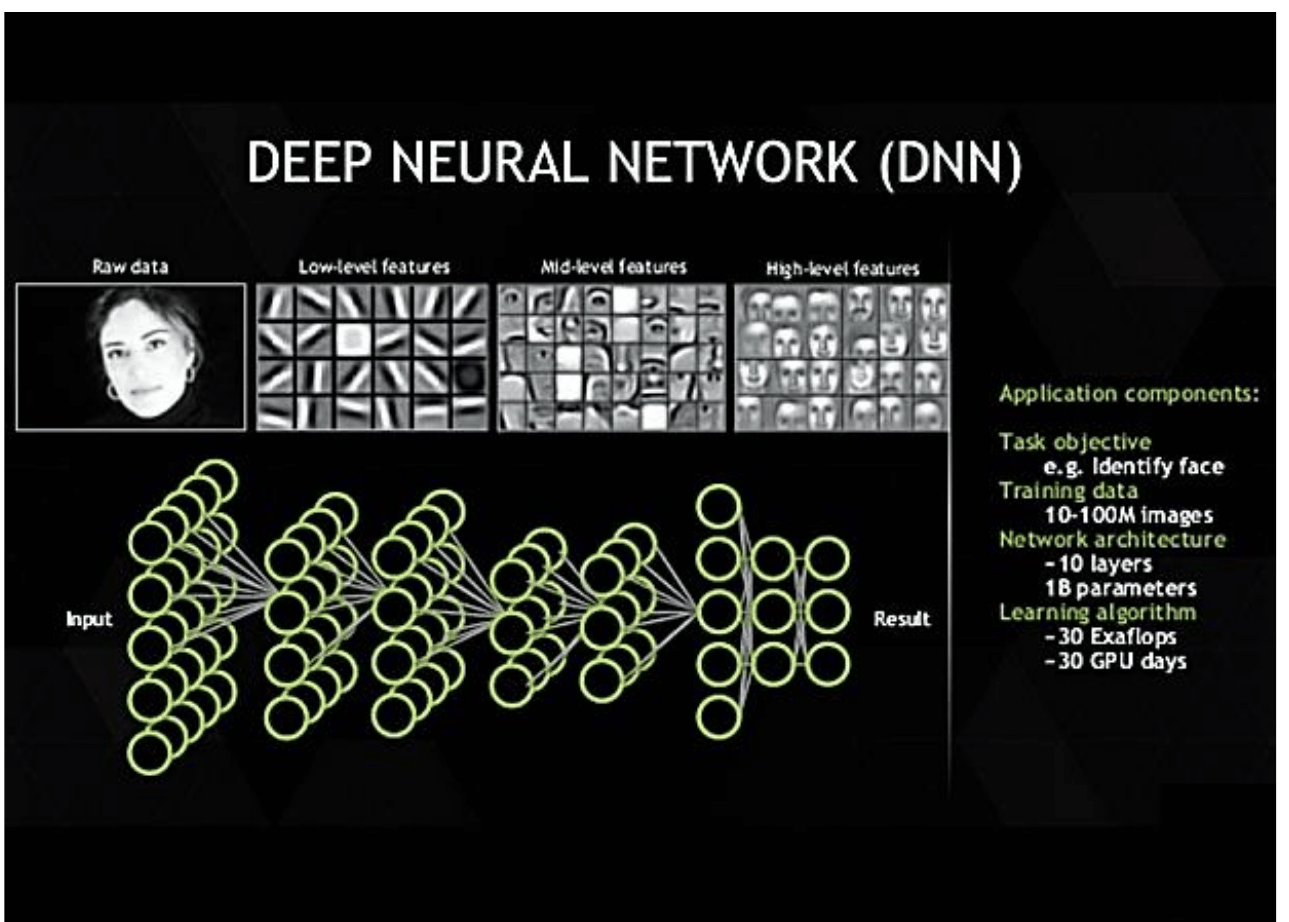
\includegraphics[width=0.69\linewidth,height=0.42\textheight,keepaspectratio]{images/17-deep_dnn.png}
\caption{Un altro esempio: feature di basso, medio e alto livello in una rete
profonda per volti.}
\end{figure}

\subsection{Combinare per
generalizzare}\label{combinare-per-generalizzare}

Le feature astratte si possono \textbf{riusare} ai livelli superiori
(es. genere, occhiali\ldots) e \textbf{combinare} per generalizzare a
casi mai visti in addestramento: se la rete ha visto donne senza
occhiali e uomini con occhiali, può rappresentare facilmente anche una
donna con gli occhiali.

\begin{figure}[htbp]
\centering
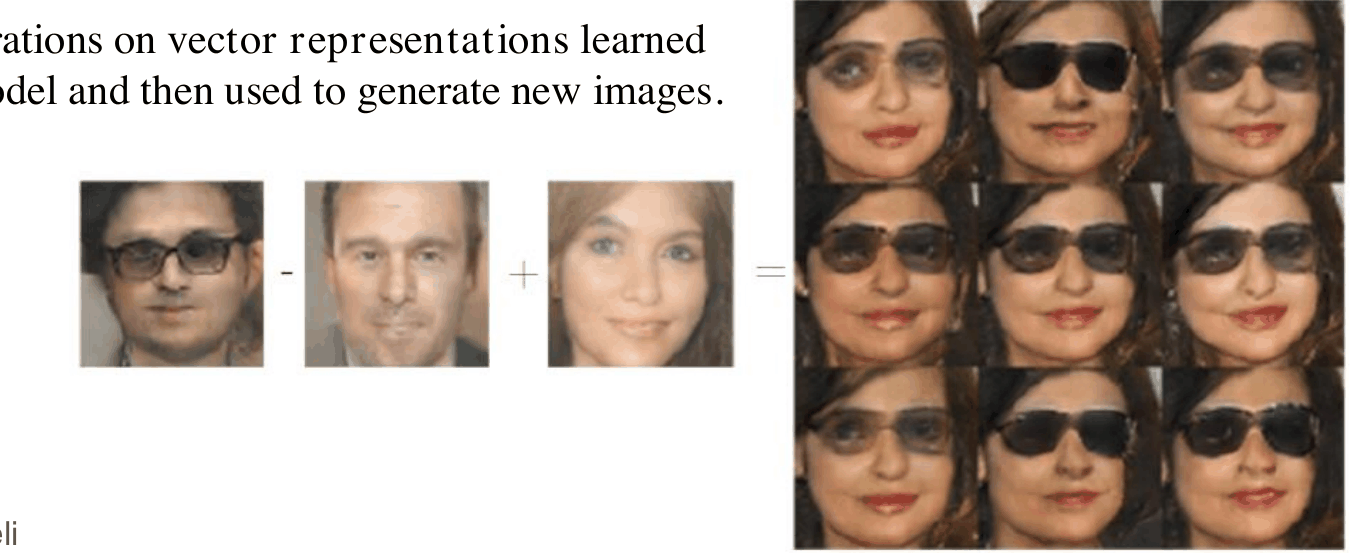
\includegraphics[width=0.74\linewidth,height=0.42\textheight,keepaspectratio]{images/17-deep_occhiali.png}
\caption{Operazioni sulle rappresentazioni vettoriali apprese dal modello e usate
per generare nuove immagini: ``uomo con occhiali − uomo + donna = donna
con occhiali''.}
\end{figure}

Lo stesso accade nel linguaggio: nello spazio vettoriale sviluppato
dagli strati interni di un modello profondo,

\begin{itemize}
\tightlist
\item
  \(\text{Rep}(\text{re}) - \text{Rep}(\text{maschio}) + \text{Rep}(\text{femmina}) \approx \text{Rep}(\text{regina})\):
  la differenza tra ``re'' e ``maschio'' cattura il concetto di
  monarchia;
\item
  \(\text{Rep}(\text{Parigi}) - \text{Rep}(\text{Francia}) + \text{Rep}(\text{Polonia}) \approx \text{Rep}(\text{Varsavia})\):
  la differenza cattura il concetto di capitale.
\end{itemize}

\section{Servono davvero molti
strati?}\label{servono-davvero-molti-strati}

\subsection{Un esempio dai circuiti
logici}\label{un-esempio-dai-circuiti-logici}

L'idea generale (\textbf{no-flattening}): \emph{quando una funzione si
rappresenta in modo compatto con un'architettura profonda, potrebbe
richiedere un'architettura molto grande per essere rappresentata con una
insufficientemente profonda.}

Un circuito logico a \textbf{due strati} può rappresentare
\textbf{qualsiasi} funzione booleana, scritta come somma di prodotti
(forma normale disgiuntiva): porte AND nel primo strato (con eventuale
negazione degli input) e una porta OR nel secondo. Ma \textbf{con
circuiti di profondità due, la maggior parte delle funzioni booleane
richiede un numero esponenziale di porte} (rispetto alla dimensione
dell'input).

\begin{boxexample}{La funzione di parità}

La \textbf{parità dispari} estende lo XOR a \(N\) input: restituisce 1
se e solo se il numero di 1 tra gli \(N\) bit è dispari. (Si assume di
disporre anche dei NOT; con 2 input bastano 3 porte.)

\textbf{Con 2 strati} bisogna elencare tutte le configurazioni positive:
per 3 input,
\(x_1x_2x_3 + x_1\bar x_2\bar x_3 + \bar x_1x_2\bar x_3 + \bar x_1\bar x_2x_3\)
(1 se l'input è 111, 100, 010 o 001), cioè 4 AND + 1 OR = 5 porte. Per 4
input servono 9 porte, per 8 input \textbf{129 porte}, per \(N\) input
\(2^N/2 + 1 = 2^{N-1} + 1\) porte: un numero \textbf{esponenziale}.

\textbf{Con \(\log N\) strati} si usa un \textbf{albero binario
completo} di XOR: un albero con \(N\) foglie ha \(N - 1\) nodi interni,
ognuno uno XOR da 3 porte AND/OR, per un totale di \(3(N-1)\) porte, un
numero \textbf{polinomiale}. Per 8 input bastano \(3 \times 7 = 21\)
porte contro le 129 della soluzione a 2 strati.

\end{boxexample}

\begin{figure}[htbp]
\centering
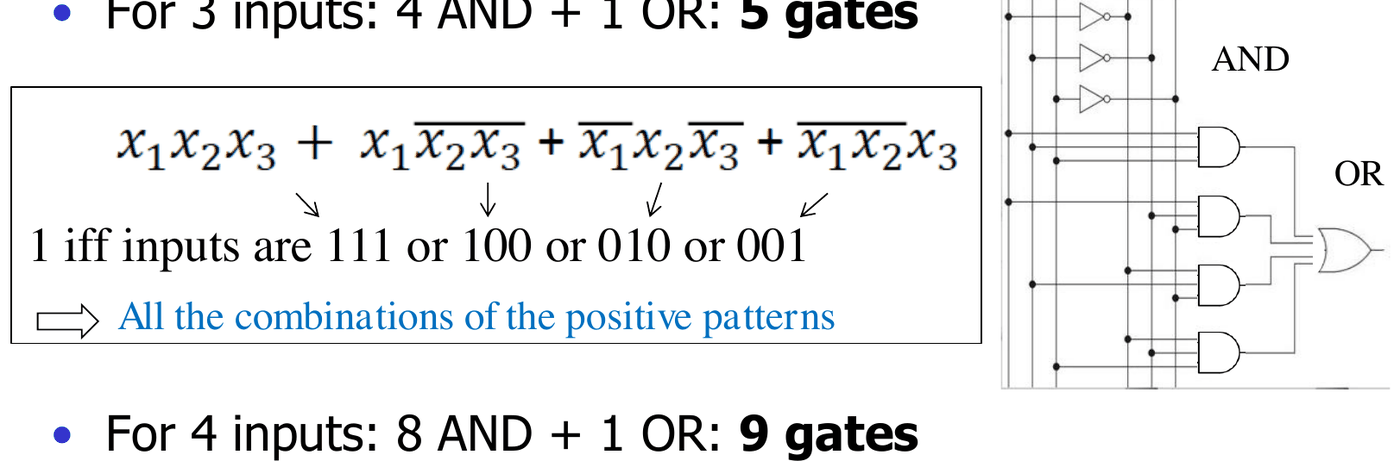
\includegraphics[width=0.80\linewidth,height=0.42\textheight,keepaspectratio]{images/17-deep_parita-2strati.png}
\caption{Parità con 2 strati: un numero esponenziale di porte.}
\end{figure}

\begin{figure}[htbp]
\centering
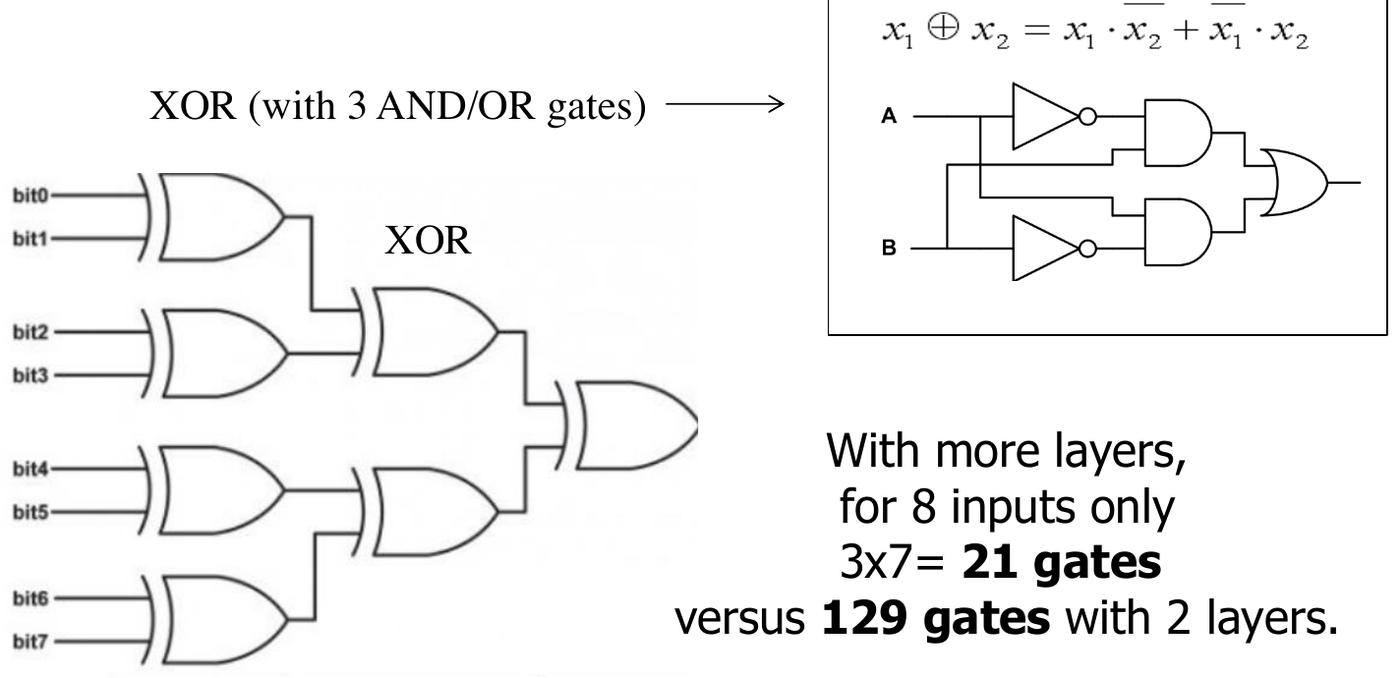
\includegraphics[width=0.74\linewidth,height=0.42\textheight,keepaspectratio]{images/17-deep_parita-albero.png}
\caption{Parità con \(\log N\) strati: un albero di XOR con un numero polinomiale
di porte.}
\end{figure}

Questo però \textbf{non vale per tutte le classi di funzioni}:
caratterizzare le classi che traggono un vantaggio (esponenziale) da una
struttura a più strati è un problema di ricerca aperto.

\subsection{Il caso delle reti
neurali}\label{il-caso-delle-reti-neurali}

Ricordiamo che il \textbf{teorema di approssimazione universale} mostra
che uno strato nascosto basta in generale, ma non garantisce che basti
un numero \textbf{piccolo} di unità. Esistono però risultati di
\textbf{no-flattening} (sull'efficienza, non sull'espressività):

\begin{enumerate}
\def\labelenumi{\arabic{enumi}.}
\tightlist
\item
  \textbf{reti shallow}: ci sono casi in cui l'implementazione con un
  solo strato nascosto richiede un numero \textbf{esponenziale} di unità
  (rispetto alla dimensione \(n\) dell'input) o di pesi non nulli. È
  facile vederlo nel caso binario: le funzioni booleane su \(\{0,1\}^n\)
  sono \(2^{2^n}\), e nel caso peggiore può servire un'unità nascosta
  per ogni configurazione di input da distinguere (come nell'esempio
  della parità). Non è solo un problema di dimensione della rete:
  significa anche che diventa \textbf{difficile apprendere con pochi
  esempi} (ed è questo il punto più rilevante per il ML);
\item
  \textbf{no-flattening delle reti profonde}: esistono famiglie di
  funzioni approssimabili in modo efficiente con profondità maggiore di
  \(d\), ma che richiedono un modello molto più grande (fino a un
  guadagno esponenziale) se la profondità è al più \(d\). Esempi per
  porte logiche (1986), reti con attivazioni standard (1990--1994), ReLU
  (2014)\ldots{}
\end{enumerate}

Resta la domanda: è facile addestrare un MLP con molti strati? (Vedi le
tecniche più avanti.)

\begin{boxnote}{Analisi teorica (ricerca aperta)}

I \textbf{teoremi di no-flattening} individuano funzioni composizionali
che una rete profonda implementa bene e che non si possono implementare
con la stessa efficienza ``appiattendo'' la rete (ad esempio passando da
un numero lineare a uno esponenziale di unità). Ma non c'è garanzia che
un dato task abbia questa proprietà: un elenco completo dei teoremi di
no-flattening direbbe esattamente quando le reti profonde sono più
efficienti di quelle superficiali.

\end{boxnote}

\subsection{Perché: la
composizionalità}\label{perchuxe9-la-composizionalituxe0}

Le reti profonde possono sfruttare la \textbf{composizionalità delle
rappresentazioni interne}: c'è un guadagno esponenziale di potere
rappresentativo perché i concetti semplici rappresentati in uno strato
vengono usati come \textbf{primitive} dallo strato successivo per
rappresentare concetti più complessi, evitando la rappresentazione (e
l'apprendimento) esplicita e combinatoria delle feature.

Ad esempio, si devono imparare le singole parole o sotto-pattern, ma non
direttamente tutte le loro possibili combinazioni: si può imparare senza
vedere tutte le configurazioni. E forse la natura stessa (non solo
immagini e linguaggio) ha una struttura gerarchica (fenomeni osservati a
scale diverse nello spazio e nel tempo).

\begin{boxtip}{Meno è meglio!}

Non bisogna vedere le reti profonde come modelli \textbf{enormi}
rispetto a piccoli modelli superficiali (solo perché nelle applicazioni
si vedono istanze gigantesche: profondo non significa grande). Si
possono vedere come modelli \textbf{compatti} rispetto a modelli
superficiali potenzialmente molto più grandi per lo stesso task (anche
esponenzialmente). Quindi sono ``qualcosa di meno'' e più efficienti. E
non solo per ragioni computazionali: \textbf{meno unità e meno pesi
aiutano l'apprendimento} su task complessi, permettendo di generalizzare
bene con \textbf{meno esempi} (cioè rendendolo fattibile). Una ``piccola
rete profonda'' da 50.000 unità può sostituire una ``enorme rete
superficiale'' da un milione di unità.

\end{boxtip}

\subsection{Il bias induttivo}\label{il-bias-induttivo}

Scegliere un modello profondo codifica una \textbf{convinzione molto
generale}: che la funzione da apprendere sia una \textbf{composizione di
funzioni più semplici} (o di fattori di variazione annidati). Se il task
corrisponde a questo bias, la forma profonda è adatta, e la
generalizzazione risulta migliore proprio grazie ai molti strati.

Task tipicamente gerarchici: la struttura delle \textbf{immagini}
(composizione di parti grafiche), la struttura del \textbf{linguaggio}
(testo e parlato), forse la musica; nuovi campi si stanno scoprendo. Ma
non necessariamente tutti i dati e i task! È comunque un bias molto più
\textbf{generale} di vincoli ad hoc per task specifici (come le \(\phi\)
scelte a mano nelle LBE o le feature ingegnerizzate). Ma, di nuovo,
nulla è magico senza assunzioni.

\begin{figure}[htbp]
\centering
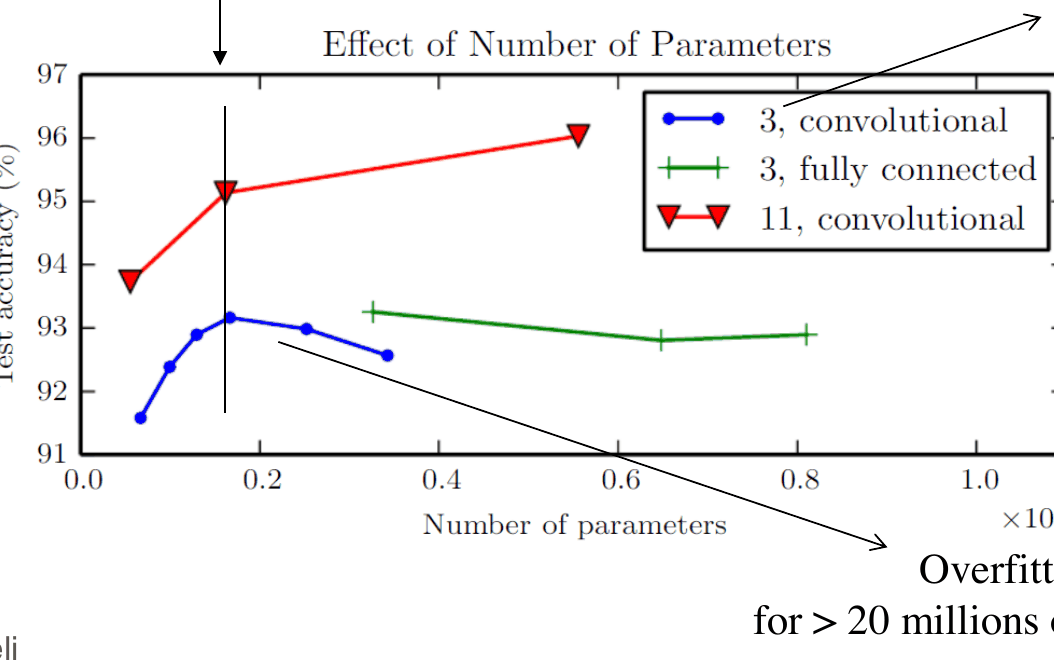
\includegraphics[width=0.57\linewidth,height=0.42\textheight,keepaspectratio]{images/17-deep_svhn.png}
\caption{Risultati empirici (SVHN, ICLR 2014): a parità di numero di parametri,
le reti più profonde generalizzano meglio.}
\end{figure}

Quando il task corrisponde al bias, i modelli più profondi tendono a
funzionare meglio: la generalizzazione è migliore di un modello con meno
strati e \textbf{lo stesso numero di unità/pesi}.

\subsection{Maledizione della dimensionalità e
bias}\label{maledizione-della-dimensionalituxe0-e-bias}

Altri argomenti a favore dei modelli profondi riguardano la
\textbf{curse of dimensionality} e il \emph{manifold learning} (la
distribuzione delle immagini e dei testi reali sembra concentrata su una
varietà che occupa solo una piccola frazione del volume di tutte le
possibili immagini o testi casuali).

\begin{itemize}
\tightlist
\item
  Molti learner si basano su \textbf{approssimazioni locali} (un prior
  di \emph{smoothness} locale): K-NN, kernel locali, alberi di
  decisione\ldots{} Ma spesso questo non basta: servono esempi per
  generalizzare nell'intorno di ogni regione, e in alta dimensione
  servono moltissimi esempi per coprire tutto lo spazio. Per distinguere
  \(O(k)\) regioni, tutti questi metodi richiedono \(O(k)\) esempi.
\item
  Per lavorare con \(O(k)\) esempi su un numero \textbf{esponenziale}
  (in \(k\)) di regioni, cioè per generalizzare \textbf{non localmente},
  servono ipotesi aggiuntive sulla distribuzione che genera i dati (un
  bias induttivo).
\item
  Si potrebbero fare ipotesi forti e specifiche per ogni task (perdendo
  generalità). Il deep learning sceglie invece un bias
  \textbf{generale}, legato alla \textbf{composizione di funzioni}: si
  assume che i dati siano generati dalla composizione di fattori o
  feature, potenzialmente su più livelli di una gerarchia. Quando
  l'ipotesi è vera, si ottiene un guadagno potenzialmente esponenziale
  tra numero di esempi e numero di regioni distinguibili, si generalizza
  non localmente, e si impara con meno esempi.
\end{itemize}

\subsection{Questioni pratiche}\label{questioni-pratiche}

Quanti strati? Quante unità? Non c'è ancora una risposta generale (è un
problema di model selection). In generale le reti profonde usano spesso
meno unità per strato, quindi meno parametri e meno dati per
generalizzare bene; ma molti strati possono essere \textbf{più difficili
da ottimizzare}. Gli iperparametri di questi modelli molto grandi
possono essere troppi: l'\textbf{esperienza} fa la differenza nel
fissare molti aspetti architetturali.

\section{Representation learning}\label{representation-learning}

\begin{boxdefinition}{Representation learning}

\emph{``Il representation learning è un insieme di metodi che permette a
una macchina di ricevere dati grezzi e scoprire automaticamente le
rappresentazioni necessarie per il rilevamento o la classificazione.''}
(LeCun, Bengio, Hinton, 2015)

\end{boxdefinition}

I metodi di deep learning sono metodi di representation learning con
\textbf{più livelli} di rappresentazione (rappresentazioni espresse in
termini di altre più semplici). Ma il concetto è più astratto e vale per
molti modelli (ad esempio le reti neurali in generale). Si noti che si
parla di apprendere la rappresentazione soprattutto per \textbf{dati
grezzi} (immagini, stringhe di testo), non quando si fornisce già un
piccolo insieme di feature.

\subsection{Idee di base}\label{idee-di-base}

\begin{itemize}
\tightlist
\item
  Molti compiti di elaborazione dell'informazione sono facili o
  difficilissimi \textbf{a seconda di come l'informazione è
  rappresentata} (vale in tutta l'informatica).
\item
  Nel ML, \textbf{una buona rappresentazione è quella che rende più
  facile il compito di apprendimento successivo}.
\item
  Progettare le feature a mano è difficile: interi decenni di lavoro per
  alcune comunità (linguaggio, immagini). Equivale a ingegnerizzare a
  mano le \(\phi(\mathbf{x})\) della LBE.
\item
  L'apprendimento supervisionato di un MLP porta a una
  \textbf{rappresentazione automatica} in ogni strato nascosto, con
  proprietà che rendono più facile il compito dello strato di uscita (lo
  XOR!). Cioè \(\phi(\mathbf{x}, \mathbf{w})\) viene appresa trovando il
  miglior \(\mathbf{w}\).
\item
  Nelle CNN si usa l'immagine grezza come input e il modello impara a
  estrarre le feature salienti per il task, senza pattern o feature
  specificati in anticipo.
\end{itemize}

Come ottenere o sfruttare le rappresentazioni nascoste (oltre
all'addestramento completo di MLP e CNN)?

\begin{itemize}
\tightlist
\item
  \textbf{Ottenerle} (caso storico): con l'apprendimento
  \textbf{semi-supervisionato} si impara una rappresentazione dai dati
  non etichettati e la si usa per task supervisionati →
  \textbf{pre-training}.
\item
  \textbf{Sfruttarle}: la rappresentazione appresa si usa per altri task
  → \textbf{transfer learning}.
\end{itemize}

\subsection{Pre-training}\label{pre-training}

Il \emph{greedy layer-wise unsupervised pretraining} (circa 2006) fu il
primo approccio che rese possibile addestrare reti supervisionate
profonde (a parte CNN e RNN). Si usa l'apprendimento \textbf{non
supervisionato} per catturare la forma della distribuzione dell'input,
\textbf{strato per strato}, e si inizializza così la rete, rendendo più
facile l'addestramento complessivo (anziché fare subito un addestramento
\emph{end-to-end} con la discesa del gradiente, che per i modelli
profondi era difficile).

Perché aiuta? Ogni strato è ottimizzato indipendentemente in modo non
supervisionato, costituendo un pre-addestramento per il
\textbf{fine-tuning} finale. Funziona sia come \textbf{buona strategia
di inizializzazione} sia come \textbf{regolarizzazione}: non nel senso
di un modello più semplice, ma di scoprire feature che catturano le
regolarità dei dati. Se le funzioni vere sono complicate e modellate
dalle regolarità della distribuzione degli input, l'apprendimento non
supervisionato può essere un regolarizzatore più appropriato. Riduce
anche la \textbf{varianza} del processo di stima (i modelli
pre-addestrati tendono a finire in una regione più piccola).

\subsubsection{Autoencoder}\label{autoencoder}

\begin{boxdefinition}{Autoencoder}

Un \textbf{autoencoder} è una rete neurale addestrata a \textbf{copiare
il proprio input in uscita}. Internamente ha uno strato nascosto
\(\mathbf{h}\) che descrive un \textbf{codice} per rappresentare
l'input. Si compone di un \textbf{encoder}
\(\mathbf{h} = f(\mathbf{x})\) e di un \textbf{decoder} che produce la
ricostruzione \(\mathbf{r} = g(\mathbf{h})\).

\end{boxdefinition}

\begin{figure}[htbp]
\centering
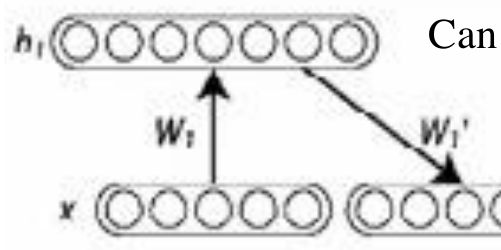
\includegraphics[width=0.34\linewidth,height=0.42\textheight,keepaspectratio]{images/17-deep_autoencoder.png}
\caption{Un autoencoder: encoder (W₁) e decoder (W₁').}
\end{figure}

\begin{itemize}
\tightlist
\item
  \textbf{Undercomplete}: lo strato nascosto è \textbf{più piccolo}
  dell'input, e il vincolo architetturale forza la rete a catturare le
  feature più salienti. (Con decoder lineare e loss quadratica si
  ottiene la PCA.)
\item
  \textbf{Overcomplete}: lo strato nascosto è \textbf{più grande}
  dell'input, ma si usa una regolarizzazione che impone sparsità,
  robustezza al rumore o altre proprietà, oltre alla banale capacità di
  copiare.
\item
  È apprendimento \textbf{non supervisionato}.
\end{itemize}

Esempio d'uso: \textbf{denoising autoencoder} e memorie
auto-associative. Si addestra su immagini cercando una buona
rappresentazione (``\emph{una buona rappresentazione è quella che si può
ottenere in modo robusto da un input corrotto e che è utile per
recuperare l'input pulito}''), poi si recupera l'immagine originale
presentandone una versione rumorosa e ripetendo le fasi di codifica e
decodifica.

\subsubsection{L'algoritmo di pre-training
(Bengio)}\label{lalgoritmo-di-pre-training-bengio}

\begin{boxabstract}{Pre-training layer-wise}

\begin{enumerate}
\def\labelenumi{\arabic{enumi}.}
\tightlist
\item
  Addestrare il primo strato come \textbf{autoassociatore} per
  minimizzare l'errore di ricostruzione dell'input grezzo (non
  supervisionato: bastano esempi non etichettati).
\item
  Usare le uscite delle unità nascoste come input per un altro strato,
  anch'esso addestrato come autoassociatore.
\item
  Ripetere fino al numero di strati desiderato.
\item
  Usare l'uscita dell'ultimo strato nascosto come input per uno strato
  supervisionato, inizializzato (casualmente o con addestramento
  supervisionato, tenendo fisso il resto).
\item
  \textbf{Fine-tuning} di tutti i parametri rispetto al criterio
  supervisionato.
\end{enumerate}

Si spera che l'inizializzazione non supervisionata abbia portato i
parametri in una regione da cui la discesa locale raggiunge un buon
ottimo locale.

\end{boxabstract}

Gli autoencoder si usano come RBM (\emph{Restricted Boltzmann Machines},
modelli basati sull'energia, nelle \emph{deep belief network} di Hinton)
o come autoencoder (denoising) impilati (Bengio, 2007).

\begin{boxnote}{Serve ancora il pre-training?}

Il pre-training ha permesso di \textbf{far partire} il deep learning e
dà ancora miglioramenti in alcuni task (soprattutto NLP, dove permette
di sfruttare grandi corpora di testo per apprendere rappresentazioni
distribuite delle parole). Ma è difficile da gestire (iperparametri
divisi in due fasi) e oggi \emph{``il pre-training non supervisionato è
largamente abbandonato''} (DL book, cap. 15): le tecniche moderne
bastano per un buon addestramento \textbf{end-to-end} da zero con la
backpropagation.

\end{boxnote}

\begin{boxnote}{Encoder e decoder oggi}

\begin{itemize}
\tightlist
\item
  Gli \textbf{autoencoder variazionali} usano un quadro bayesiano: lo
  spazio latente è una miscela di distribuzioni invece di un vettore
  fisso.
\item
  La \textbf{traduzione automatica neurale} si realizza con architetture
  encoder-decoder in cui l'uscita non coincide con l'input ma è in
  un'altra lingua.
\item
  I \textbf{transformer} (come GPT, \emph{Generative Pre-trained
  Transformer}) sono reti encoder/decoder con un meccanismo di
  \textbf{attenzione}. Si può usare solo l'encoder (BERT, per vari task
  NLP) o solo il decoder, a scopo generativo (la serie GPT per la
  generazione autoregressiva di testo).
\end{itemize}

\end{boxnote}

\subsection{Transfer learning}\label{transfer-learning}

Si usa la rappresentazione scoperta da un modello per \textbf{migliorare
un altro modello}, assumendo che esistano feature utili in contesti o
task diversi, corrispondenti a fattori sottostanti comuni. Forme diverse
(sono veri sotto-campi del ML, non solo terminologia):

\begin{itemize}
\tightlist
\item
  dall'autoencoder al classificatore (come sopra);
\item
  \textbf{multi-task learning}: stessi input, target diversi (una
  regolarizzazione implicita);
\item
  \textbf{domain adaptation}: dominio di input diverso ma feature
  condivise (es. analisi del sentiment su recensioni di video e di
  smartphone);
\item
  riuso di \textbf{modelli pre-addestrati} su dataset più grandi.
\end{itemize}

\begin{boxexample}{Transfer learning con AlexNet}

AlexNet è una CNN addestrata su circa 1,2 milioni di immagini ImageNet
in 1000 categorie: ha appreso \textbf{rappresentazioni ricche} per
un'ampia gamma di immagini, con primitive di basso livello condivise tra
immagini diverse. Ha 5 strati convoluzionali e 3 completamente connessi.
Per un nuovo task si \textbf{sostituiscono gli ultimi 3 strati} e si
addestrano solo quelli con poche immagini nuove, oppure si fa il
\textbf{fine-tuning} di tutta la rete. Molte CNN pre-addestrate (VGG,
ResNet, GoogLeNet\ldots) sono disponibili nelle librerie.

\end{boxexample}

\section{Rappresentazioni
distribuite}\label{rappresentazioni-distribuite}

\begin{boxdefinition}{Rappresentazione distribuita}

\emph{``In una rappresentazione distribuita gli elementi (le feature)
non sono mutuamente esclusivi e le loro molte configurazioni
corrispondono alle variazioni osservate nei dati.''} (LeCun, Bengio,
Hinton, 2015)

\end{boxdefinition}

I metodi di deep learning sfruttano rappresentazioni distribuite su più
livelli, ma il concetto vale per molti modelli (reti neurali in
generale, sulle unità nascoste; modelli grafici probabilistici, con più
variabili latenti).

\begin{figure}[htbp]
\centering
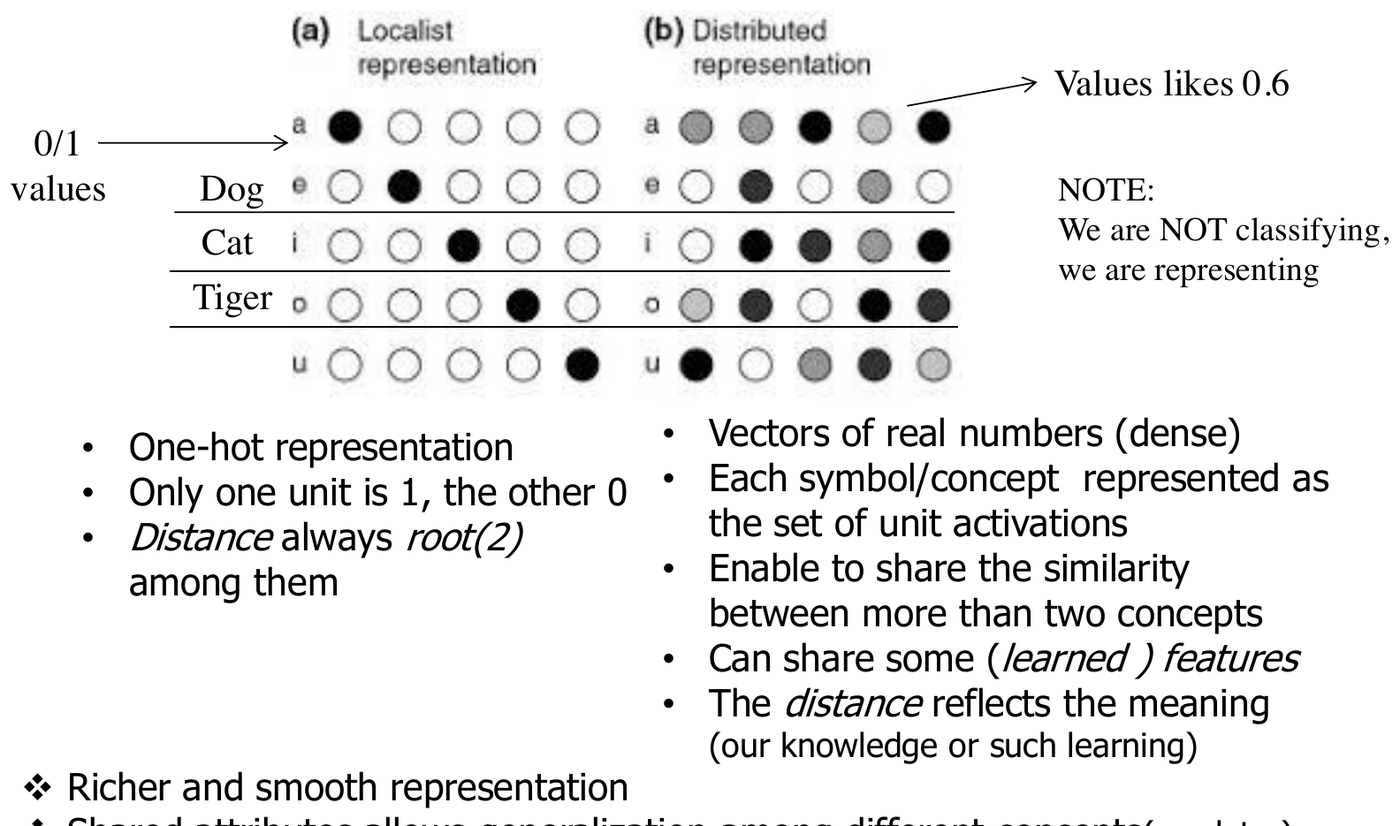
\includegraphics[width=0.74\linewidth,height=0.42\textheight,keepaspectratio]{images/17-deep_distribuita.png}
\caption{Rappresentazione simbolica (one-hot) e distribuita.}
\end{figure}

{\def\LTcaptype{none} % do not increment counter
\begin{longtable}[]{@{}
  >{\raggedright\arraybackslash}p{(\linewidth - 2\tabcolsep) * \real{0.5000}}
  >{\raggedright\arraybackslash}p{(\linewidth - 2\tabcolsep) * \real{0.5000}}@{}}
\toprule\noalign{}
\begin{minipage}[b]{\linewidth}\raggedright
Simbolica (one-hot)
\end{minipage} & \begin{minipage}[b]{\linewidth}\raggedright
Distribuita
\end{minipage} \\
\midrule\noalign{}
\endhead
\bottomrule\noalign{}
\endlastfoot
una sola unità vale 1, le altre 0 & vettori di numeri reali (densi) \\
distanza sempre \(\sqrt{2}\) tra concetti diversi & ogni concetto è
l'insieme delle attivazioni di tutte le unità \\
& la similarità si può condividere tra più di due concetti \\
& si possono condividere feature (apprese) \\
& la distanza riflette il significato \\
\end{longtable}
}

Attenzione: qui \textbf{non si classifica}, si \textbf{rappresenta}. Le
rappresentazioni distribuite sono più ricche e lisce, e gli attributi
condivisi permettono di generalizzare tra concetti diversi.

\textbf{Input o rappresentazione interna?} Il discorso è generale, ma
l'apprendimento agisce sulla rappresentazione \textbf{interna}. Una
rappresentazione distribuita in \textbf{input} si usa solo se la
conoscenza di dominio permette di fissarla (raro e difficile; fissarla
arbitrariamente può danneggiare il task). In genere si usa comunque un
input one-hot (non informato) e si lascia che il modello sviluppi
\textbf{internamente} la rappresentazione distribuita necessaria.

\subsection{Contare la differenza}\label{contare-la-differenza}

Quattro concetti: auto blu, bici blu, auto rossa, bici rossa. Non
servono 4 neuroni: ne bastano \textbf{2} (\(2^2\) concetti), uno per
blu/rosso e uno per auto/bici. E il neurone che descrive il ``rosso''
impara il rosso da immagini sia di auto sia di bici, non solo da una
specifica categoria.

In generale, con \(n\) feature a \(k\) valori una rappresentazione
distribuita descrive \(k^n\) concetti diversi (ad esempio \(2^n\)
configurazioni binarie), contro gli \(n\) di una rappresentazione
simbolica one-hot. Si può assegnare un codice unico a un numero
\textbf{esponenziale} di regioni: i modelli con rappresentazioni
distribuite (come le reti con unità nascoste) distinguono
esponenzialmente più regioni di quelli non distribuiti.

Modelli basati su rappresentazioni \textbf{non distribuite}: K-NN (uno o
pochi prototipi per input, senza condividere informazione con tutto il
training set), kernel RBF (si riducono al K-NN, come visto per le SVM),
miscele di gaussiane, alberi di decisione (si attiva una sola foglia).

\subsection{Attributi condivisi: separare i
concetti}\label{attributi-condivisi-separare-i-concetti}

\begin{figure}[htbp]
\centering
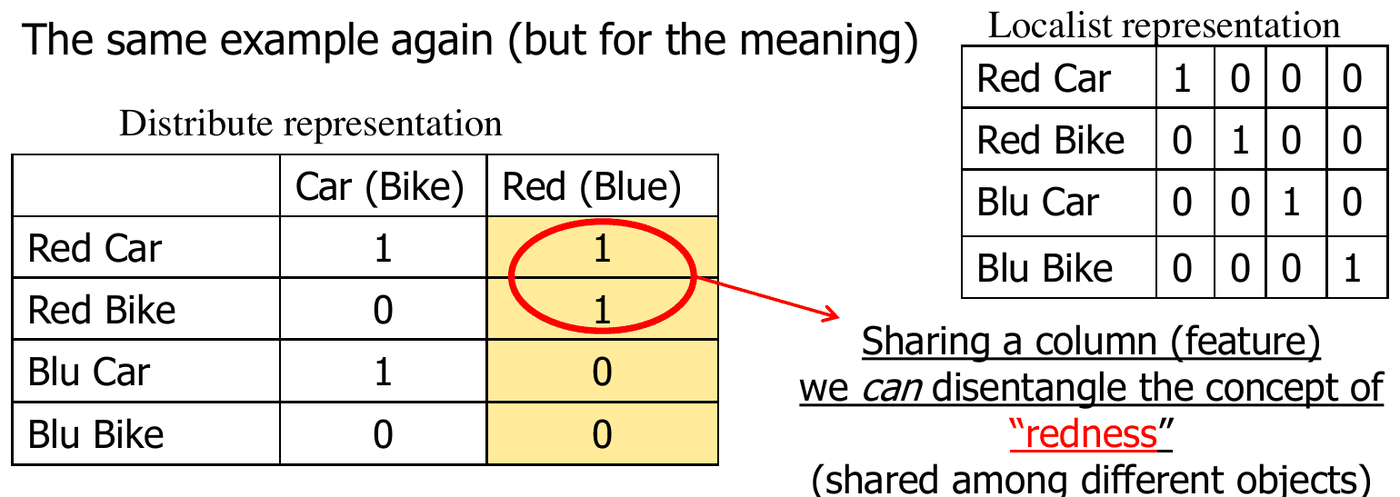
\includegraphics[width=0.80\linewidth,height=0.42\textheight,keepaspectratio]{images/17-deep_disentangling.png}
\caption{Condividendo una colonna (feature) si separa (}
\end{figure}

Separando i concetti colore e tipo, si può imparare la distinzione
auto/bici o il colore \textbf{senza dover vedere esempi di tutte le
combinazioni}. Questa \textbf{separabilità statistica} rende facile
generalizzare a configurazioni mai viste: avendo visto gli altri tre
casi, si classifica facilmente la bici blu (ad esempio ``non mi piace''
perché non è rossa, se il modello ha imparato che mi piacciono gli
oggetti rossi); con la rappresentazione localista la bici blu sarebbe
del tutto nuova.

Con le \textbf{parole}: invece di un simbolo one-hot per parola
(dimensione pari al vocabolario), una rappresentazione distribuita in
cui ``cane'' e ``gatto'' condividono feature permette al modello di:

\begin{enumerate}
\def\labelenumi{\arabic{enumi}.}
\tightlist
\item
  \textbf{trattarli in modo simile}: le frasi con ``gatto'' informano le
  predizioni per le frasi con ``cane'' e viceversa, trasferendo
  informazione da ogni frase di training a un numero esponenziale di
  frasi semanticamente affini (ad esempio ``entrambi hanno la coda'' →
  animale, non umano);
\item
  \textbf{imparare automaticamente che sono simili}, avvicinandone le
  rappresentazioni perché compaiono in contesti simili: è il
  \textbf{word embedding} (ad esempio \emph{word2vec}). Nello spazio
  one-hot ogni parola è a distanza \(\sqrt{2}\) da tutte le altre; nello
  spazio appreso parole con significato simile diventano vicine.
\end{enumerate}

\begin{figure}[htbp]
\centering
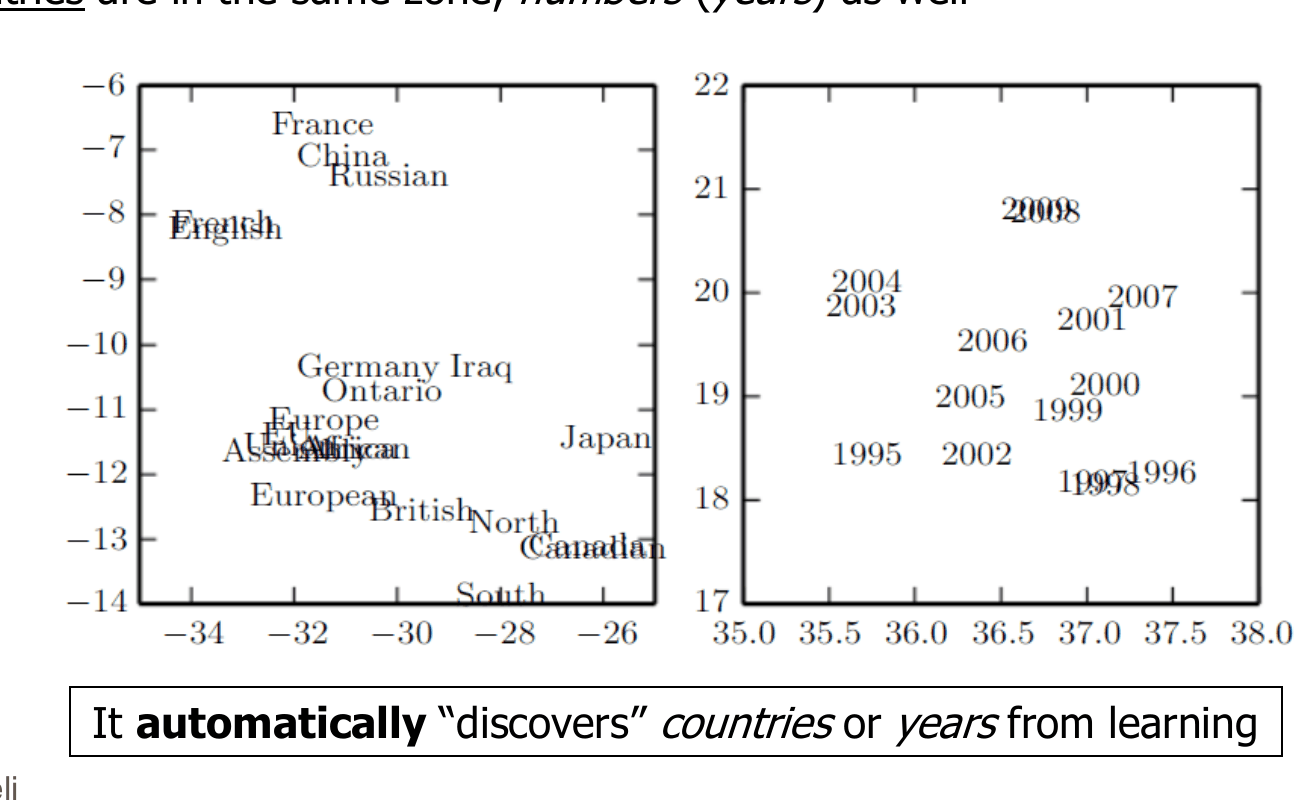
\includegraphics[width=0.69\linewidth,height=0.42\textheight,keepaspectratio]{images/17-deep_word-embedding.png}
\caption{Word embedding: parole semanticamente simili (paesi, anni) finiscono
vicine. Il modello ``scopre'' automaticamente paesi e anni
dall'apprendimento.}
\end{figure}

\begin{boxtip}{Una considerazione sui risultati}

Il modello impara non solo la grammatica (non sorprende) ma
rappresentazioni \textbf{semanticamente significative}, e lo fa
automaticamente, solo leggendo testo. Perché la nostra semantica
coincide con ciò che la rete impara? Probabilmente il linguaggio (e le
immagini) hanno intrinsecamente una struttura \textbf{gerarchica} e la
rete profonda ha il bias induttivo giusto per apprenderla in modo
distribuito (le immagini reali sono una frazione minuscola delle
immagini di rumore bianco). È ancora un campo aperto.

\end{boxtip}

Il dibattito sulle rappresentazioni distribuite si estende a quello tra
paradigmi \textbf{logico-simbolici} e \textbf{neurali} per la
cognizione: i successi nella traduzione mettono in dubbio la necessità
di approcci simbolici per capire le frasi.

\begin{boxwarning}{Interpretabilità}

Il rovescio della medaglia: una rappresentazione distribuita è
\textbf{meno facile da interpretare} di una localista.

\end{boxwarning}

\subsection{Rappresentazioni distribuite
profonde}\label{rappresentazioni-distribuite-profonde}

Il DL sfrutta rappresentazioni distribuite \textbf{attraverso molti
strati}, ottenute componendo livelli di astrazione o una gerarchia di
feature riusate. La composizionalità porta un ulteriore guadagno
esponenziale di efficienza statistica, oltre a quello delle
rappresentazioni distribuite: \textbf{due vantaggi potenzialmente
esponenziali} rispetto ai modelli non distribuiti e superficiali. Nel
complesso, i modelli di DL imparano una rappresentazione distribuita dei
dati trovando (separando) i \textbf{fattori causali condivisi} che li
generano, su diversi livelli di astrazione.

Esempi applicativi: la combinazione di CNN e RNN per generare
\textbf{didascalie di immagini} (con un meccanismo di attenzione che si
concentra sulla parte dell'immagine relativa a ogni parola generata); la
classificazione dei \textbf{tumori della pelle} con una rete profonda
addestrata su 130.000 casi, con competenza paragonabile a quella dei
dermatologi (\emph{Nature} 2017).

\section{Altri spunti e risultati
recenti}\label{altri-spunti-e-risultati-recenti}

\begin{itemize}
\tightlist
\item
  \textbf{Smoothness tramite la struttura}: a parità di parametri, le
  reti più profonde impongono più smoothness di quelle superficiali
  (ogni strato lavora sulla superficie già liscia prodotta dal
  precedente), e sembrano apprendere meglio a parità di neuroni totali:
  vincoli di smoothness \textbf{impliciti}, anziché espliciti.
\item
  \textbf{Il puzzle del non-overfitting}: reti enormi,
  sovra-parametrizzate, capaci di azzerare l'errore di training anche su
  etichette \textbf{casuali}, eppure generalizzano. Una spiegazione: la
  discesa del gradiente impone una forma di \textbf{regolarizzazione
  implicita}, con convergenza verso la soluzione a \textbf{margine
  massimo} (Poggio et al., 2017--2019). Varianti di SGD con batch/weight
  normalization massimizzano il margine normalizzato, e perfino la
  discesa del gradiente standard massimizza il margine \(L^2\) senza
  normalizzazione o regolarizzazione esplicita.
\item
  \textbf{Double descent}: nelle CNN, ResNet e transformer, al crescere
  della dimensione del modello (o dei dati, o del tempo di
  addestramento) le prestazioni prima migliorano, poi peggiorano (la
  classica U) e poi \textbf{migliorano di nuovo} oltre la soglia di
  interpolazione (dove l'errore di training diventa quasi zero).
  L'effetto è spesso evitato con una regolarizzazione accurata; non è
  ancora pienamente compreso ed è un'importante direzione di ricerca.
  (Non necessariamente riguarda i piccoli modelli del progetto.)
\end{itemize}

\begin{figure}[htbp]
\centering
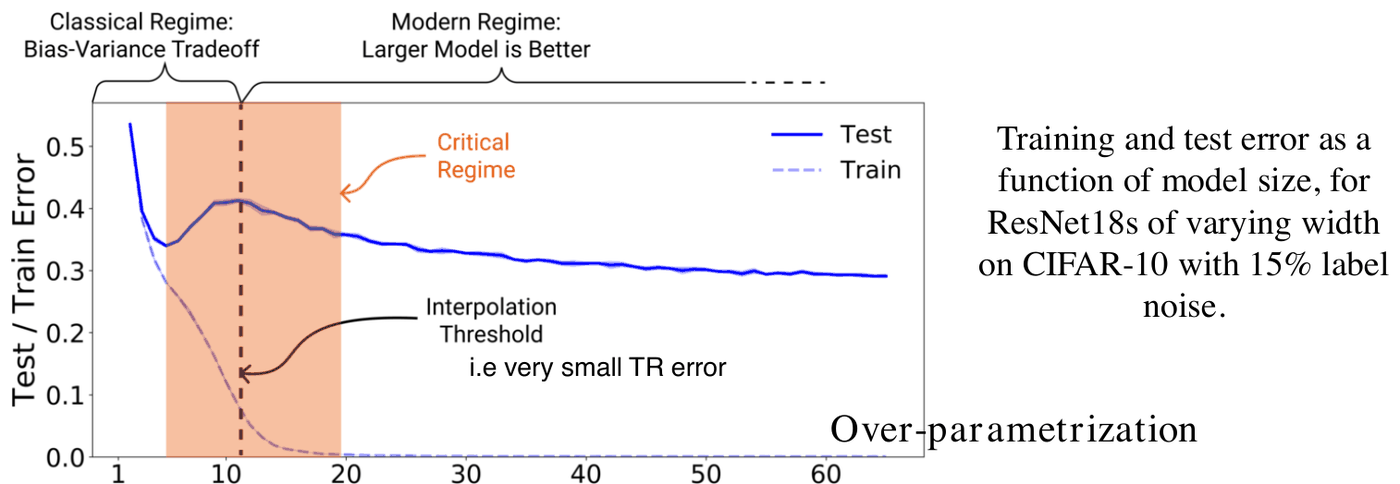
\includegraphics[width=0.80\linewidth,height=0.42\textheight,keepaspectratio]{images/17-deep_double-descent.png}
\caption{Il fenomeno del}
\end{figure}

\begin{figure}[htbp]
\centering
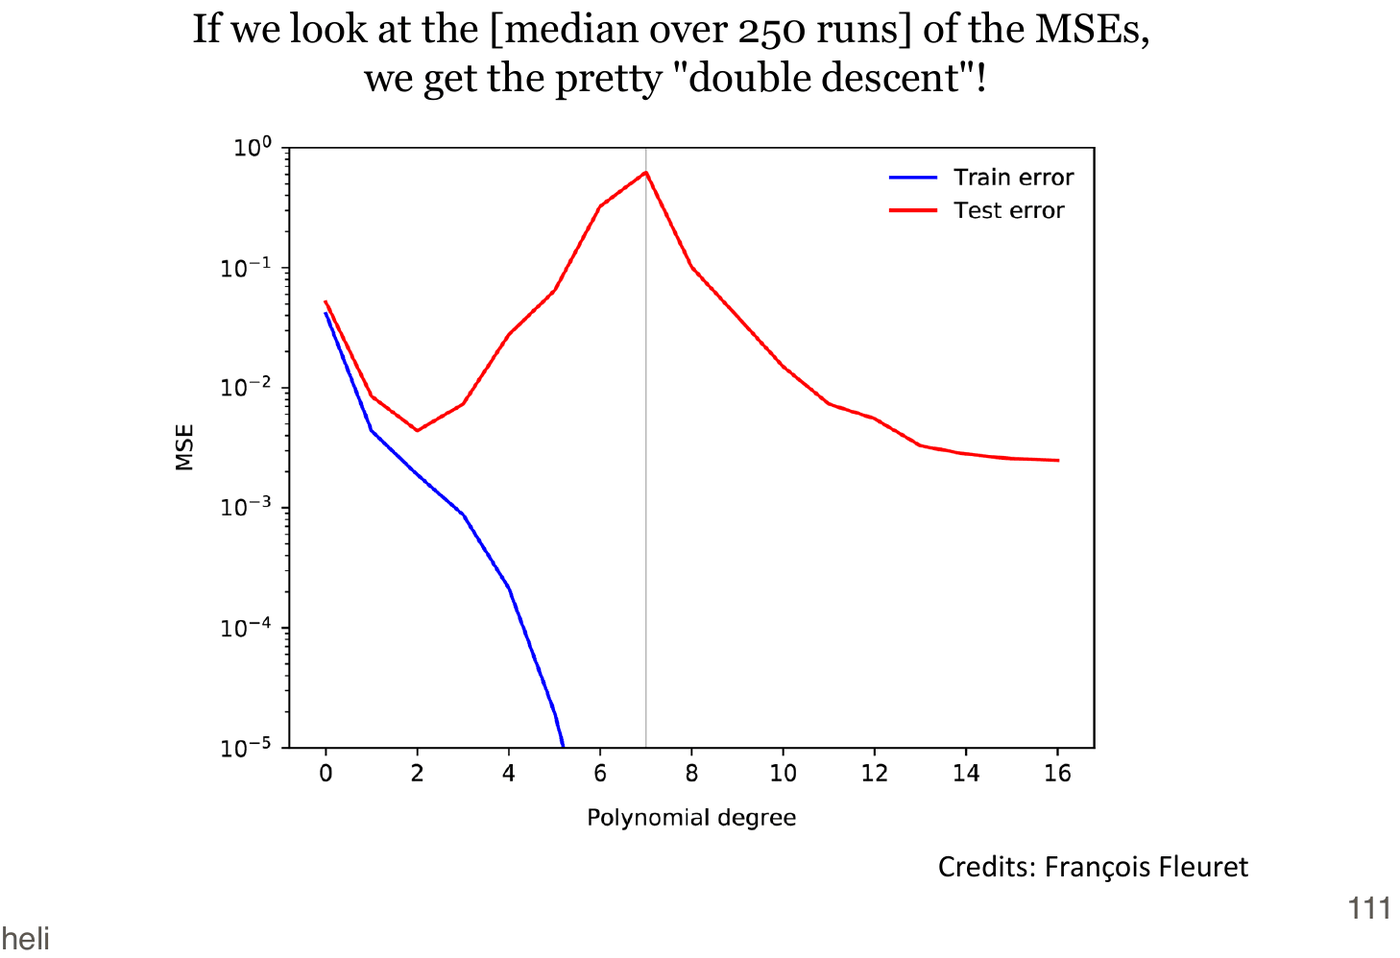
\includegraphics[width=0.54\linewidth,height=0.42\textheight,keepaspectratio]{images/17-deep_double-descent-poly.png}
\caption{Un esempio giocattolo con regressione polinomiale regolarizzata: anche
qui compare il double descent. Superato l'errore di training nullo,
all'aumentare del grado il fit è guidato solo dal termine di penalità e
il polinomio diventa sempre più ``lineare a tratti''.}
\end{figure}

\begin{itemize}
\tightlist
\item
  \textbf{Ridondanza}: nei modelli profondi c'è una ridondanza
  significativa nei parametri; dati pochi pesi per feature si possono
  predire gli altri, fino a oltre il 95\% dei pesi senza perdita di
  accuratezza (Denil et al., 2013). Si possono anche \textbf{comprimere}
  i parametri (pruning, quantizzazione, codifica di Huffman) senza
  perdite (Han et al., 2015): sembra che reti piccole bastino!
\item
  \textbf{Lottery ticket hypothesis} (Frankle e Carbin, 2018): perché
  allora addestriamo reti grandi? Perché le buone prestazioni dipendono
  da una \textbf{inizializzazione fortunata} di una o più sotto-reti, e
  le reti grandi ne contengono esponenzialmente di più. Riaddestrando la
  rete potata con la stessa inizializzazione si ottengono prestazioni
  simili.
\item
  Il ruolo della \textbf{casualità} (reti inizializzate casualmente e
  reti a pesi casuali) riceve sempre più attenzione (vedi
  \href{18\%20-\%20Reti\%20neurali\%20randomizzate}{18 - Reti neurali
  randomizzate}).
\end{itemize}

\section{Tecniche}\label{tecniche}

Molti strati possono essere difficili da ottimizzare, quindi l'enfasi è
sui metodi per migliorare la \textbf{discesa del gradiente} (anche
contro il \emph{vanishing gradient}), la \textbf{regolarizzazione} (reti
grandi) e lo \textbf{sfruttamento dei dati} (semi-supervisionato,
reinforcement learning, multi-task, apprendimento avversario\ldots). A
questo si aggiungono dataset più grandi, infrastrutture software
pubbliche e miglioramenti hardware.

\begin{boxabstract}{Tecniche chiave per il DL}

\begin{itemize}
\tightlist
\item
  In origine: approcci di \textbf{pre-training} (ancora usati in domini
  come l'NLP per i word embedding).
\item
  Oggi (nelle librerie più diffuse), in gran parte già note:

  \begin{itemize}
  \tightlist
  \item
    \textbf{SGD con momentum} (con decadimento di \(\eta\), mini-batch)
    o \textbf{Adam};
  \item
    attivazioni \textbf{ReLU} nelle unità nascoste;
  \item
    loss di \textbf{massima verosimiglianza} (cross-entropy) con
    \textbf{softmax} in uscita (anche per evitare saturazione e
    gradienti piccoli);
  \item
    regolarizzazione: early stopping, weight decay, \textbf{dropout},
    \textbf{batch normalization}.
  \end{itemize}
\end{itemize}

\end{boxabstract}

\subsection{Problemi del gradiente}\label{problemi-del-gradiente}

Cosa succede alla norma del gradiente quando lo si retropropaga
attraverso molti strati?

\begin{itemize}
\tightlist
\item
  se i pesi sono \textbf{piccoli}, i gradienti \textbf{si riducono
  esponenzialmente} (\emph{vanishing gradient}), anche per via della
  derivata delle sigmoidi;
\item
  se i pesi sono \textbf{grandi}, i gradienti \textbf{crescono
  esponenzialmente} (\emph{exploding gradient}).
\end{itemize}

\subsubsection{Il vanishing gradient}\label{il-vanishing-gradient}

Le attivazioni tradizionali come la tanh hanno gradienti in \((-1, 1)\),
e la backpropagation calcola i gradienti con la regola della catena
ripetuta attraverso gli strati. In una rete a \(d\) strati si
moltiplicano \(d\) di questi numeri piccoli per calcolare i gradienti
degli strati vicini all'input: il gradiente (il delta) \textbf{decresce
esponenzialmente con \(d\)} e gli strati vicini all'input si addestrano
lentissimamente.

\begin{boxnote}{Schizzo formale}

Se \(\mathbf{h}_l = F_l(\mathbf{h}_{l-1})\) e
\(F = F_M \circ \dots \circ F_1\), allora \[
\frac{\partial F}{\partial w_l} = \frac{\partial F_M}{\partial \mathbf{h}_{M-1}}\cdots\frac{\partial F_l}{\partial w_l}, \qquad \left|\frac{\partial F}{\partial w_l}\right| \approx \rho^{M-l+1} \text{ se } \left\|\frac{\partial F_i}{\partial \mathbf{h}_i}\right\| \approx \rho.
\] Con \(\rho < 1\) il gradiente svanisce, con \(\rho > 1\) esplode.

\end{boxnote}

Gli approcci per affrontarlo vanno da R-prop alle connessioni
\emph{shortcut}, fino alle reti randomizzate, e alle ReLU.

\subsubsection{Gradient clipping}\label{gradient-clipping}

La moltiplicazione ripetuta attraverso gli strati può introdurre
\textbf{scogliere} (\emph{cliff}) nella funzione di costo: derivate
altissime che ``catapultano'' i pesi lontanissimo. Il \textbf{clipping}
limita la norma del gradiente mantenendone la direzione: \[
\text{se } \|\mathbf{g}\| > v \;\text{ allora }\; \mathbf{g} \leftarrow \frac{v\,\mathbf{g}}{\|\mathbf{g}\|},
\] con \(v\) soglia sulla norma.

\begin{figure}[htbp]
\centering
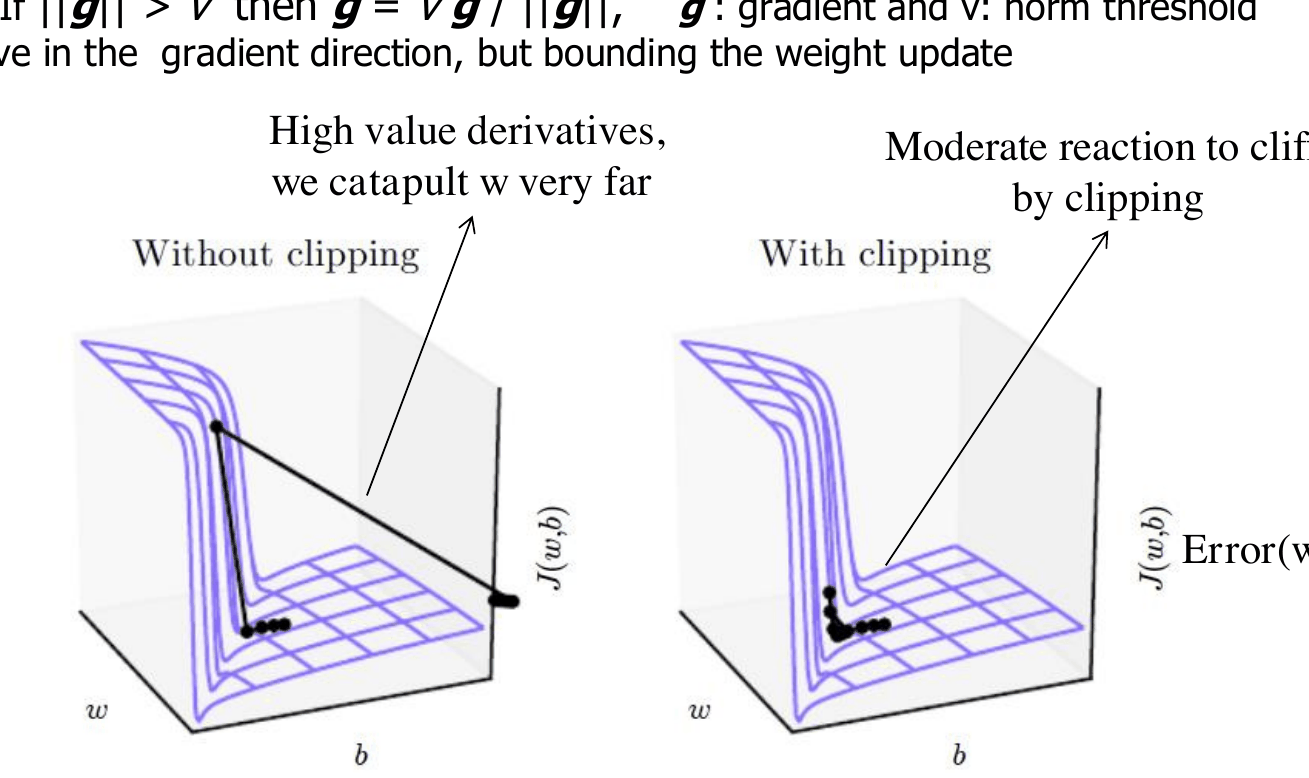
\includegraphics[width=0.69\linewidth,height=0.42\textheight,keepaspectratio]{images/17-deep_clipping.png}
\caption{Senza clipping (sinistra) e con clipping (destra) di fronte a una
scogliera della funzione di costo.}
\end{figure}

\subsection{ReLU}\label{relu}

\begin{boxdefinition}{ReLU (\emph{Rectified Linear Unit})}

\[
f(x) = \max(0, x) = \begin{cases} 0 & x < 0 \\ x & x \ge 0. \end{cases}
\]

\end{boxdefinition}

Perché usarla nel DL (dal 2009)?

\begin{itemize}
\tightlist
\item
  \textbf{Propagazione del gradiente} migliore attraverso molti strati:
  evita la saturazione delle sigmoidi, perché \(f'(x) = 1\) per ogni net
  positivo.
\item
  \textbf{Attivazione sparsa}: in una rete inizializzata casualmente
  circa il 50\% delle unità nascoste è attivo (uscita non nulla).
\item
  \textbf{Calcolo efficiente}: solo confronti, somme e prodotti.
\item
  Ha ancora un'ispirazione neuroscientifica, e permette un addestramento
  più veloce ed efficace delle reti profonde.
\end{itemize}

La ReLU \textbf{non è differenziabile in 0}, ma nelle librerie si assume
di solito derivata 0 (sinistra) o 1 (destra): l'approssimazione è
accettabile e sicura, perché per le approssimazioni numeriche è
improbabile valutare esattamente \(f(0)\). (Un approccio più rigoroso
usa l'ottimizzazione non differenziabile per funzioni lineari a tratti.)

Un trucco: iniziare con \textbf{net positivi}, ad esempio con bias
piccoli e positivi (0,1), così che le ReLU siano inizialmente attive per
la maggior parte degli input e lascino passare le derivate.

Varianti: \textbf{ELU} (\emph{Exponential Linear Unit}),
\(f(x) = \alpha(e^x - 1)\) per \(x \le 0\) e \(x\) per \(x > 0\);
\textbf{Leaky ReLU}, \(f(x) = 0{,}01x\) per \(x < 0\) e \(x\) per
\(x \ge 0\). Imparano anche sulla parte sinistra (i neuroni non si
``spengono'') e hanno attivazione media più vicina a zero. Molte
varianti hanno prestazioni comparabili; in generale evitano alcuni
difetti mantenendo la parte lineare, che rende il modello più facile da
ottimizzare.

\subsection{Batch normalization}\label{batch-normalization}

La \textbf{batch normalization} normalizza ogni mini-batch calcolandone
le statistiche (media e varianza) per ogni strato: si normalizza la
matrice {[}esempi del batch × attivazioni delle unità{]} a media zero e
varianza unitaria, e la trasformazione è inclusa nella backpropagation.
Come normalizzare l'input è pratica standard, così la BN mantiene
normalizzati i dati che fluiscono tra gli strati intermedi. Effetti:
\textbf{regolarizzazione} (per il rumore introdotto dal mini-batch) e
\textbf{apprendimento più rapido} con accuratezza più alta (rilevante
perché ha permesso di addestrare efficacemente CNN e modelli profondi
con sigmoidi). (Dettagli non richiesti all'esame, a meno di usarla.)

\subsection{Dropout}\label{dropout}

Il \textbf{dropout} seleziona casualmente un sottoinsieme della rete
durante l'addestramento. Si spiega con due concetti già noti:
\textbf{ensemble} (un bagging implicito di sotto-reti diverse, ma
computazionalmente economico) e \textbf{regolarizzazione}.

Il bagging addestra \(n\) modelli su sottoinsiemi diversi del training
set e ne media le uscite: modelli ad alta varianza e basso bias
funzionano bene in media. Il dropout approssima e sfrutta questo
processo con un numero \textbf{esponenziale} di sotto-reti, pur avendo a
test time \textbf{una sola rete}, e massimizza la diversità
dell'ensemble evitando co-adattamenti complessi sui dati di training.

\begin{figure}[htbp]
\centering
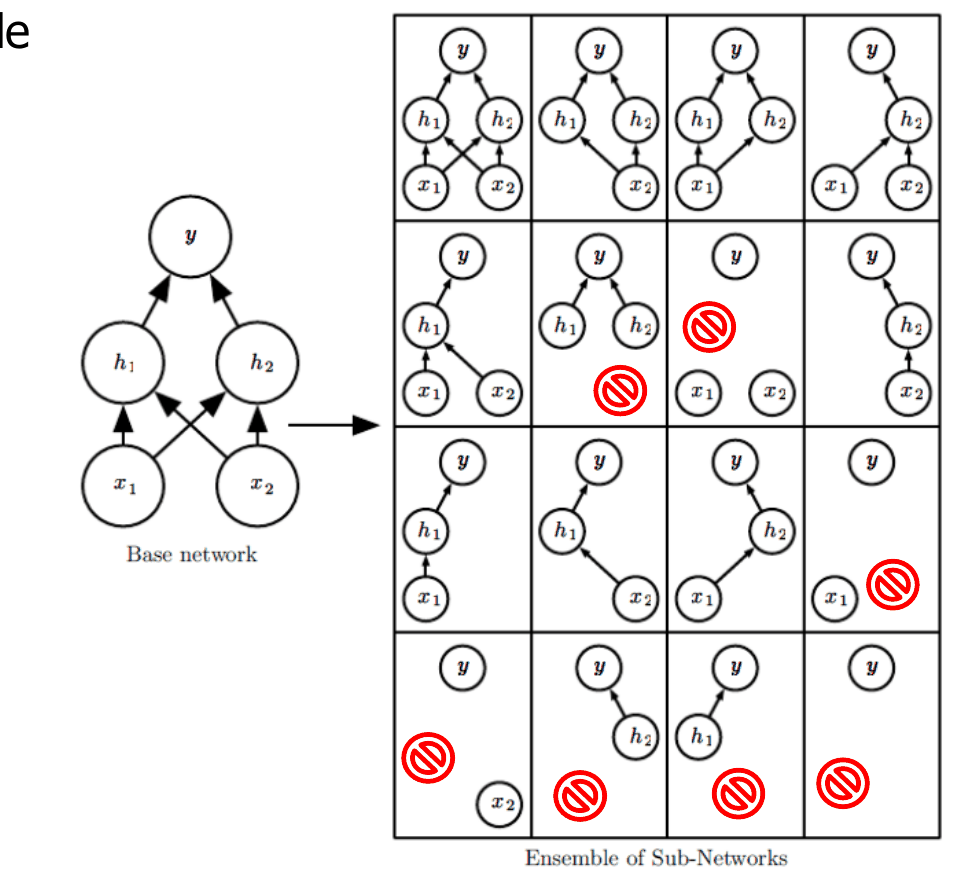
\includegraphics[width=0.51\linewidth,height=0.42\textheight,keepaspectratio]{images/17-deep_dropout.png}
\caption{Il dropout addestra l'ensemble di tutte le sotto-reti ottenibili
rimuovendo unità non di uscita dalla rete base. Alcune sotto-reti non
funzionano, ma in reti grandi è improbabile che non ci sia alcun
percorso dall'input all'uscita.}
\end{figure}

\begin{boxabstract}{Algoritmo del dropout}

\begin{itemize}
\tightlist
\item
  Ogni volta che si carica un esempio in un mini-batch, si campiona una
  diversa \textbf{maschera binaria} da applicare a tutte le unità di
  input e nascoste, indipendentemente per ogni unità. La probabilità di
  includere un'unità è un iperparametro (tipicamente 0,8 per l'input e
  0,5 per le unità nascoste).
\item
  Ogni unità viene moltiplicata per la sua maschera (zero equivale a
  rimuoverla, \emph{drop out}): si ottiene una sotto-rete.
\item
  Si eseguono forward, backpropagation e aggiornamento come al solito,
  addestrando un sottoinsieme di unità alla volta.
\item
  Le unità rimosse vengono poi reinserite con i loro pesi originali.
\end{itemize}

\end{boxabstract}

Solo una piccola frazione delle sotto-reti viene addestrata (ciascuna
per un solo passo), ma la \textbf{condivisione dei parametri} fa sì che
anche le altre arrivino a buoni parametri: si gestisce un numero
esponenziale di modelli con memoria trattabile. Per approssimare la
predizione dell'ensemble a test time si usa la \emph{weight scaling
inference rule}: si moltiplicano i pesi per la probabilità di inclusione
(tipicamente 0,5), così che l'uscita attesa di ogni unità sia la stessa
dell'addestramento.

Effetto regolarizzante: evita di addestrare tutte le unità su tutti i
dati riducendone le interazioni (e diversificandole, come serve ai
comitati); riduce la varianza come il bagging; inserisce \textbf{rumore
strutturato} (ad esempio riconoscere un volto senza l'unità che rileva
il naso). Soprattutto, regolarizza ogni unità a essere non solo una
buona feature, ma \textbf{una feature buona in molti contesti}
(sotto-reti diverse). Per la regressione lineare equivale al weight
decay \(L^2\) con un \(\lambda\) diverso per ogni input. Si può usare
con qualsiasi modello a rappresentazione distribuita addestrato con SGD.

\subsection{Regolarizzazione L1}\label{regolarizzazione-l1}

Usare la norma \(L^1\) (somma dei valori assoluti) al posto della
\(L^2\) nella penalità (per i modelli lineari è il \textbf{LASSO})
favorisce l'\textbf{eliminazione} di feature (pesi esattamente a zero),
mentre la \(L^2\) di solito riduce solo la grandezza dei pesi: si
ottengono modelli più semplici. La soluzione richiede tecniche di
ottimizzazione non differenziabile (sub-gradiente, approssimazioni lisce
della norma \(L^1\)\ldots).

\begin{figure}[htbp]
\centering
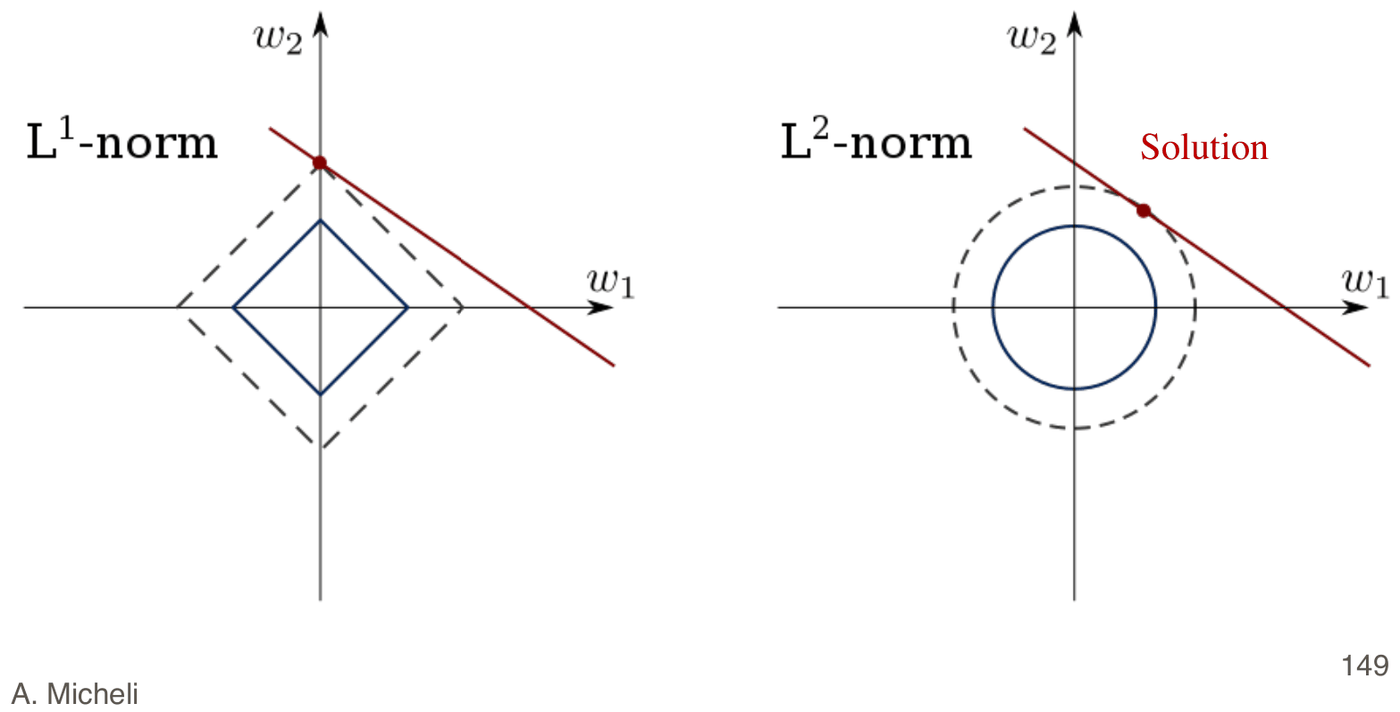
\includegraphics[width=0.74\linewidth,height=0.42\textheight,keepaspectratio]{images/17-deep_l1-l2.png}
\caption{Perché L1 produce soluzioni sparse: le curve di livello della norma L1
hanno ``spigoli'' sugli assi, dove una coordinata è nulla.}
\end{figure}

\subsection{Apprendimento avversario}\label{apprendimento-avversario}

Le \textbf{Generative Adversarial Network} (GAN) sono due reti in
competizione: una \textbf{genera} candidati, l'altra li \textbf{valuta}
(distinguendo i veri dai generati). Sono usate ad esempio per generare
immagini fotorealistiche di persone che non esistono.

\section{Applicazioni, sfide e
conclusioni}\label{applicazioni-sfide-e-conclusioni}

Il DL ha successo nell'\textbf{NLP} (riconoscimento del parlato,
traduzione, sentiment analysis, question answering\ldots), nella
\textbf{computer vision} (immagini e video: riconoscimento di oggetti,
applicazioni mediche, sintesi di immagini\ldots) con prestazioni mai
raggiunte prima, e nel gioco del \textbf{Go}. Se ne parla più a fondo
nei corsi di NLP e ISPR.

Sfide aperte: analisi e quadro teorici; progettazione ottima
dell'architettura (quanti strati? che unità? la cross-validation può
essere troppo costosa); efficienza per i big data; elaborazione di
stream (on-line); dati strutturati (sequenze, alberi, grafi).

Anche l'hardware è cambiato: TPU di Google (inizialmente solo per
l'inferenza), GPU Nvidia, NPU nei chip per smartphone (Huawei Kirin
970), il \emph{Neural Engine} di Apple (dal 2017).

\begin{boxabstract}{Sintesi}

\begin{itemize}
\tightlist
\item
  I progressi tecnici e la disponibilità di dati hanno reso possibile
  apprendere con reti profonde e molto grandi, con risultati allo stato
  dell'arte soprattutto dove la \textbf{composizionalità} delle feature
  è rilevante (visione, linguaggio).
\item
  Due vantaggi potenzialmente esponenziali: la \textbf{profondità}
  (composizione di funzioni, no-flattening) e le
  \textbf{rappresentazioni distribuite} (attributi condivisi).
\item
  Il concetto più generale emerso è il \textbf{representation learning}.
\item
  Tecniche: ReLU, cross-entropy con softmax, SGD con momentum/Adam,
  dropout, batch normalization, gradient clipping.
\item
  Il ML rende relativamente più facile sviluppare sistemi di AI (e
  software in generale) sofisticati per problemi reali.
\end{itemize}

\end{boxabstract}

\begin{boxquestion}{Possibili domande d'esame}

\begin{itemize}
\tightlist
\item
  Cosa si intende per deep learning? Quali sono gli aspetti comuni ai
  vari approcci?
\item
  Servono davvero molti strati? Discutere l'esempio della parità e i
  risultati di no-flattening.
\item
  Qual è il bias induttivo dei modelli profondi?
\item
  Cos'è il representation learning? Pre-training e transfer learning.
\item
  Cos'è un autoencoder?
\item
  Rappresentazioni simboliche contro distribuite: vantaggi delle
  seconde.
\item
  Cos'è il vanishing gradient? Come si affronta (ReLU, clipping\ldots)?
\item
  Descrivere il dropout e spiegarne l'effetto regolarizzante.
\end{itemize}

\end{boxquestion}
